\section{BACKGROUND}
In this section, we will review the MapReduce programming
model and detail the salient features of Phoenix, 
an implementation of MapReduce for multicore.
Then the limitation of Phoenix in the aspect of performance is analyzed.
%讨论Phoenix的局限与不足

\subsection{MapReduce Programing Model}
Inspired  by funnctional languages, the MapReduce programming model is 
proposed for data intensive computation in cluster environment.
Its simple programming interface require programmer 
to only define two primitives: map and reduce.
The map function is applied on the input data and 
produces a list of intermediate key and value pairs.
The reduce function is applied on all intermediate
pairs and  groups all pairs with the same key to a single
key-value pair. 
The combine function is an optional operation 
to aggregates the key and value pairs locally in Map phase 
aiming to save networking bandwidth and reduce memory consumption.


The charm of MapReduce is that, 
for applications that can fit that form, 
it hides all the concurrency details from  programmer. 
For example, 
one can count the number of occurrences for each word in a text file. 
The map function emits a $\langle word, 1\rangle$ pair for each word in document, 
and the reduce function counts all occurrences of a word as the output. 
The combine function is similar to the reduce function, 
but only processes a partial set of key-value pairs in Map phase.


\subsection{Phoenix}
Phoenix is an implementation of MapReduce for multicore  and multiprocessor systems using Pthreads\cite{}.
It shows MapReduce is a promising model  and applications written with MapReduce model
have competitive scalability and performance in comparison to those
written with Pthreads\cite{ranger2007phoenix};

Phoenix stores the intermediate key-value pairs produced 
by the Map phase calls in a global matrix (Figure \ref{fig:phoenix:intermediate}). 
Each map and reduce workers can write or read this global matrix. 
Concurrent map workers can touch the same area without synchronous controls.
When map and reduce workers operate the buffer concurrently, 
two  strategies must be carried out to avoid lock and cache contention costs,
\begin{itemize}
	\item Each row of the matrix is exclusively used by a map worker, 
and each column of the matrix is exclusively used by a reduce worker. 
	\item There is a barrier between Map and Reduce phase.
After all map workers have been completed, the reduce workers begin to compute. 
\end{itemize}


\begin{figure}[!h!t]  
    \centering
    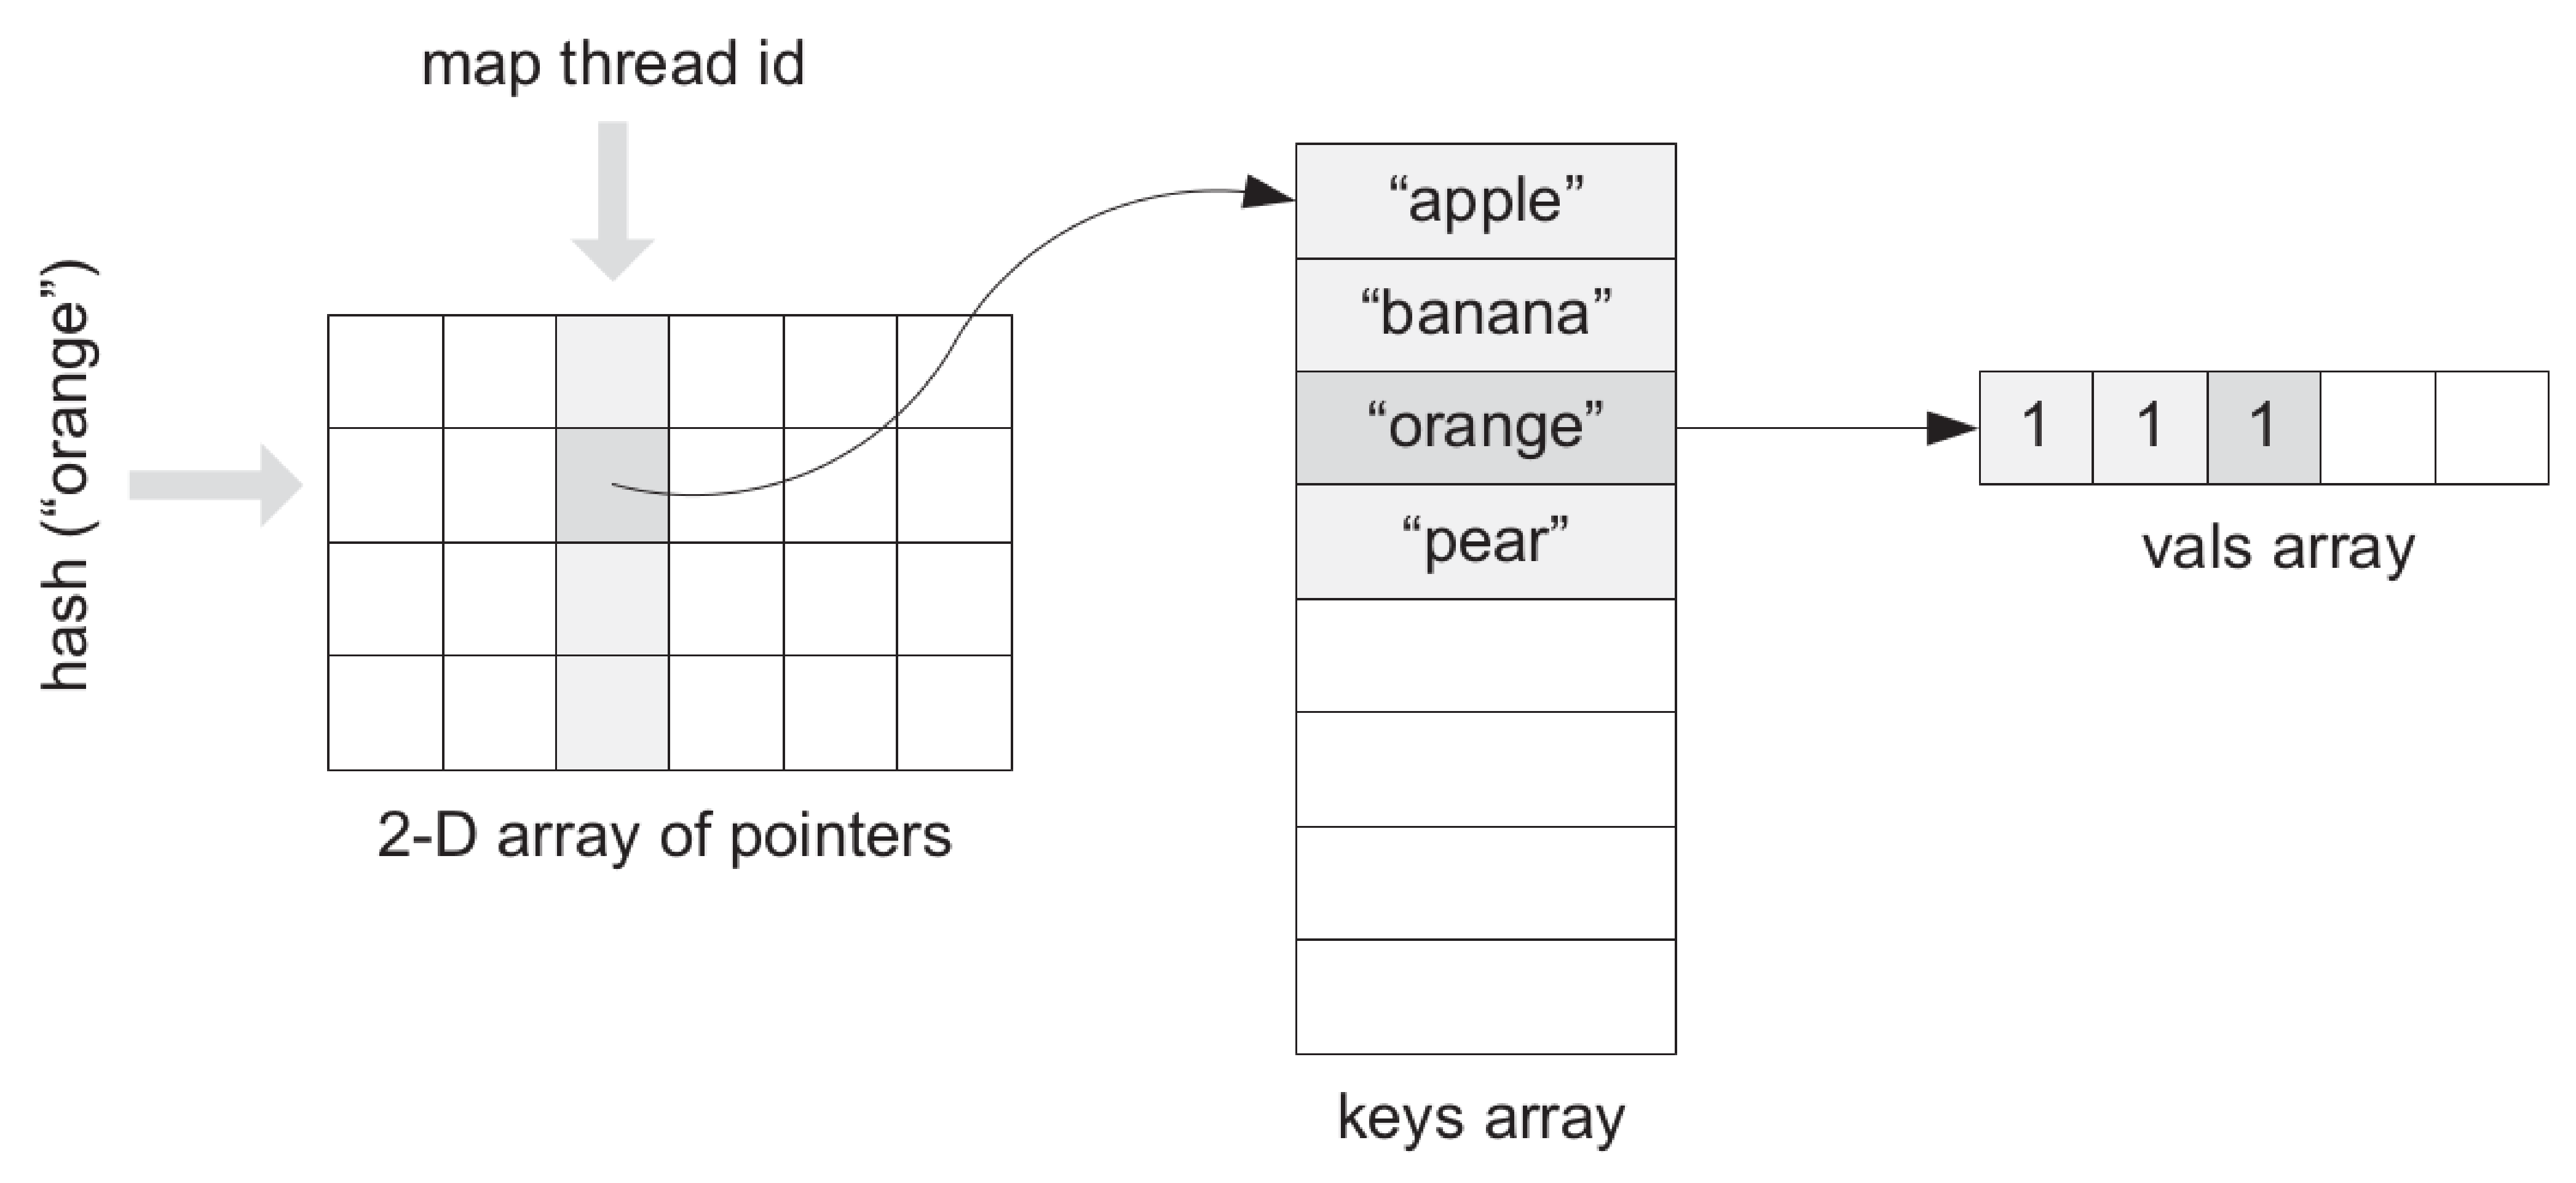
\includegraphics[width=0.45\textwidth]{eps/phoenix_intermediate.eps}
    \caption{Phoenix intermediate struct}
    \label{fig:phoenix:intermediate}
\end{figure}
%as depicted in
As shown in this figure \ref{fig:phoenix:speedup}, 
%when using no more than eight cores, the Phoenix scales well on hist ... ;
%when using no more than 16 cores, the Phoenix scales well on sm and le.
the Phoenix scales well on histgram (hist), wordcount (wc) and pca when the number of core is less than 8.
As for the linear\_regression (lr) and string\_match (sm), 
Phoenix performs well with no more than 16 cores.
However, when core number is more than  8, 
the speedup of Phoenix  on hist,  wc and pca is degraded.
For lr and sm, the speedup is degraded when cores is greater than 16.
%For linear\_regression (lr) and string\_match (sm),  using 16 or more  cores leads to speedup degradation.

%The scalability of Phoenix is limited, the performance will be
%better when the number of cores increases from 1 to 4, 
%while the performance will be worse if using more than 4 cores. 
%Perf\cite{}.\redt{need to talk more about the results...}


\begin{figure}[!h!t]  
    \centering
    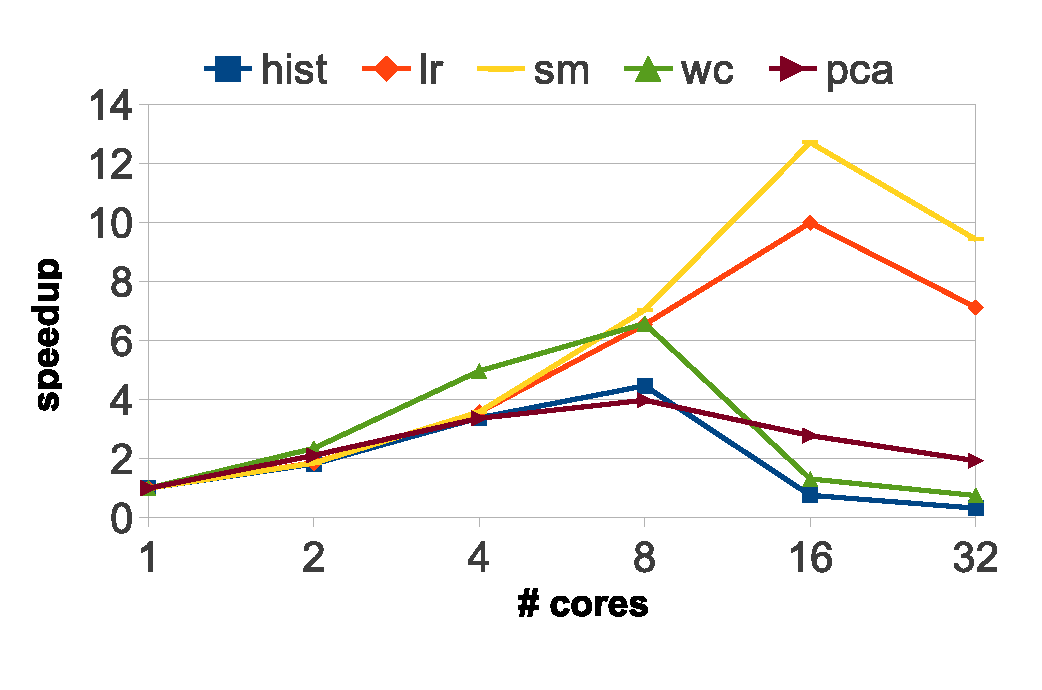
\includegraphics[width=0.45\textwidth]{eps/phoenix_speedup.eps}
    \caption{speedup of Phoenix}
    \label{fig:phoenix:speedup}
\end{figure}


\subsection{Optimizing Opportunities of Phoenix}
%Though Phoenix has successfully demonstrated the feasibility
Though Phoenix has demonstrated promising feasibility when running  applications on multicore,  it has limitations in terms of scalability and performance due to its manners of design and implementation.
The detail analyses are described as follows:
%it also has some deficiencies as increasing number of cores.
%processing jobs with a relatively large amount of threads, 

%which would be common for parallel programming with shared-memory multithreading.
First, there is a strict barrier between the Map and Reduce phase,
requiring that the workers in Reduce phase can
be started only when all workers in Map phase has been finished, 
therefore this barrier limits parallel computing.
Moreover,  the execution time of the Map phase is subjected to the slowest map worker, which means that if one of the map workers is slow, then the MapReduce will need more time.
%\bluet{If one of a map worker is slow, then the runtime of MapReduce will be need more time.} it is worth menthion that 
Furthermore, the user-defined map functions are usually computation-intensive while the Reduce phase is memory-intensive. Thus, the serialization of the Map and Reduce phase is bad for the utilization of system hardware resource.
%barrier不利于资源的利用
%由于map和reduce阶段之间存在一个barrier,只有当map worker全部结束之后,reduce才开始工作,这种严格的barrier不利于并发,并且,如果其中一个map worker花费太多时间,会让真个的运行时间变长,另一方面,由于map 是computition-intensive,而reduce是memory-intensive,Map和Reduce阶段的串序执行,不利于硬件资源的利用。

Second,  in cluster environment, network bandwidth is the key factor for performance since the map and reduce workers, executed in different machines usually,  communicate by the network.
However, when processing MapReduce applications in multicore environments,  the data structures shared by multiple threads, instead of the network, are the major performance bottlenecks.
By using the Pthreads,  a share-memory threads model, 
the threads in Phoenix require to share the process's address space.
In fact, there is a single lock for per shared address space inside the operating system’s virtual memory system. 
As a result, multithreaded applications on many-core processors suffer from serious contended locks.
This phenomenon will be common for parallel programming with shared-memory
multithreading \cite{clements2013radixvm}.

%多核环境下,限制mapreduce性能的关键因素是多线程共享的数据结构。phoenix是基于共享内存的Pthreads多线程编写的,其中每个线程没有自己独立的地址空间,它们需要共享进程的地址空间,在linux中,每个进程地址空间有一个锁对应,当多个线程需要共享时,便会对这个lock竞争,这种现象对于基于共享内存的多线程并行编程非常普片。

In conclusion, Phoenix can not achieve desired scalability with increasing core count because of the strict barrier and contented lock.
To aviod the aforementioned issues, a novel MapReduce model, \myds,  is proposed in this paper,
%employ/exploit/utilize/use
which exploits producer-consumer model to break barrier
and adopts a new thread program model to reduce lock contending.
The implementation details of \myds are presented in Section 3 and Section 4, respectively.  



%为了避免上述提到的问题,我们希望我们新设计的系统,拥有以下两个特性(1)break barrier (2),提升scalability


